\documentclass{tfg}

\usepackage[utf8]{inputenc}

\usepackage{eurosym}
\usepackage{listings}
\usepackage{caption}
\lstdefinestyle{tfgstyle}{
	captionpos=b
}
\lstset{
	basicstyle=\ttfamily,
	style=tfgstyle,
	frame=single,
	showstringspaces=false,
}

\usepackage[normalem]{ulem}
\useunder{\uline}{\ul}{}

\renewcommand*{\lstlistingname}{Cuadro}
\renewcommand*{\lstlistlistingname}{Índice de cuadros}

\tfgtitle{Migración del sistema operativo TinyCore y el software Docker a la placa computadora BeagleBoard}
\tfgdegree{Ingeniería del Software}
\tfgauthor{Alejandro Ojeda Gutiérrez}
\tfgtutor{Daniel Cagigas Muñiz}
\tfgdepartment{Arquitectura y tecnología de computadores}
\tfgdate{Septiembre, 2016}

\begin{document}

\tfgmaketitle
\cleardoublepage

\pagenumbering{roman}
\chapter*{Abstract}
The goal of this project is the migration of the minimalist operating system TinyCore to the development boards
``BeagleBoard-xM'' and ``BeagleBone Black'', as well as the pre-installation of the Docker software in this operating system
to facilitate the use of containers in such devices.
\\\par
This document describes the process followed to meet these goals, as well as the difficulties found during it's development. It also
details the process to deploy and install the TinyCore operating system and Docker software in the devices.

\chapter*{Resumen}
El objetivo de este proyecto es la migración del sistema operativo minimalista TinyCore a las placas de desarrollo
``BeagleBoard-xM'' y ``BeagleBone Black'', así como la pre-instalación del sistema Docker en dicho sistema operativo
para facilitar el uso de contenedores en dichos dispositivos.
\\\par
Este documento describe el proceso seguido para cumplir dichos objetivos, así como las dificultades halladas durante su desarrollo.
Tambien detalla el proceso para desplegar e instalar el sistema operativo TinyCore y el software Docker en los dispositivos.

\tableofcontents
\lstlistoflistings
\listoffigures

\cleardoublepage
\pagenumbering{arabic}

\chapter{Definición de objetivos}
El proyecto tiene los siguientes objetivos:
\begin{itemize}
	\item Adaptar y compilar TinyCore para las placas ``BeagleBoard-xM'' y ``BeagleBone Black''.
	\item Compilar y pre-instalar Docker en el sistema operativo.
	\item Describir el proceso para crear contenedores de Docker que funcionen en los dispositivos.
\end{itemize}

\chapter{Análisis}
\section{Tecnologías usadas}
\subsection{TinyCore}
TinyCore es un sistema operativo basado en Linux que ofrece una base extremadamente minimalista y flexible para
integrar aplicaciones. Su filosofía de reducir el sistema operativo al mínimo y maximizar su rendimiento es
fácilmente visible en su elección de BusyBox como shell o en su decisión de copiarse y residir en la RAM del dispositivo
desde el inicio del proceso de arranque para minimizar el acceso a disco. \cite{tinycore}

Se ha decidido utilizar TinyCore debido a que es código abierto, a que es muy flexible en lo que respecta a configuración,
a que esta bien documentado y a que consume pocos recursos en comparación con otras distribuciones, dejando el máximo posible
a Docker y los contenedores que corran en el.
\begin{figure}[hb]
	\centering
	
\includegraphics[scale=0.8]{images/tinycore_logo}
	\caption{Logotipo de TinyCore}
\end{figure}


\subsection{Docker}
Docker es una herramienta diseñada para facilitar la creación y uso de contenedores. Un contenedor contiene una o varias
aplicaciones así como todas las librerías y demás artefactos necesarios para su ejecución, garantizando así que la
aplicación funcione en cualquier sistema Linux sin importar la versión de las aplicaciones y librerías ya instaladas, con la única
excepción del kernel, que sí se comparte con el contenedor. \cite{docker}
\\\par
Al contrario que una máquina virtual que emula todo el sistema, Docker solo virtualiza el sistema de archivos,
permitiendo así el máximo rendimiento.
\begin{figure}[hb]
	\centering
	
\includegraphics[scale=0.75]{images/docker_logo}
	\caption{Logotipo de Docker}
\end{figure}

\subsection{Crosstool-NG}
Crosstool-NG es una herramienta diseñada para facilitar la construcción de ``toolchains'' para la cross-compilación de
aplicaciones a otras arquitecturas. En este proyecto se utilizará para crear el ``toolchain'' que se usará para compilar
el kernel, BusyBox y el resto de programas escritos en C para la arquitectura de nuestro dispositivo. \cite{crosstoolng}

\section{Análisis temporal y de costes}
A continuación se detallan los costes temporales y económicos del proyecto. Cabe destacar que la mayoría del tiempo de la implementación se ha usado resolviendo problemas debidos a diferencias de versiones, arquitecturas, etc, o problemas específicos al dispositivo (e.g. resolver problemas de arranque sin acceso a la consola serie).

Nótese que el coste económico es aproximado debido a que los materiales fueron proporcionados en su totalidad por la universidad.
\\
\begin{center}
\captionof{table}{Costes temporales del proyecto}
\begin{tabular}{ll}
{\ul \textbf{Tarea}}                                                                  & {\ul \textbf{Horas}} \\
\\
\textbf{Implementación}                                                               &                      \\
Análisis de tecnologías y búsqueda de documentación & 8h                   \\
Diseño de la solución                                                                 & 6h                   \\
Búsqueda y descarga de los componentes                                                & 3h                   \\
\\
\textit{Implementación de la construcción y despliegue de los siguientes componentes:} &                      \\
Kernel de Linux                                                                       & 1h                   \\
Toolchain                                                                             & 5h                   \\
EGLibC                                                                                & 1h                   \\
BusyBox                                                                               & 1h                   \\
Sudo                                                                                  & 1h                   \\
UDev                                                                                  & 2h                   \\
IPTables                                                                              & 1h                   \\
Docker                                                                                & 16h                  \\
WPA Supplicant                                                                        & 2h                   \\
Base de TinyCore                                                                      & 3h                   \\
Despliegue en tarjeta SD                                                              & 1h                   \\
\\
Creación de los scripts de construcción                                               & 3h                   \\
Resolución de problemas referentes a la librería EGLibC                                & 16h                  \\
Resolución de problemas referentes al arranque de la BeagleBone Black                  & 8h                   \\
Resolución de problemas referentes al soporte de WiFi                                  & 8h                   \\
{\ul \textit{\textbf{SUBTOTAL:}}}                                                     & 86h                  \\
\\
\textbf{Documentación}                                                                &                      \\
Elaboración de la memoria                                                             & 40h                  \\
Elaboración de la presentación                                                        & 10h                  \\
{\ul \textit{\textbf{SUBTOTAL:}}}                                                     & 50h                  \\
\\
{\ul \textbf{TOTAL:}}                                                                 & 136h
\end{tabular}
\end{center}

\begin{minipage}{\textwidth}
\begin{center}
\captionof{table}{Costes económicos del proyecto}
\begin{tabular}{lr}
{\ul \textbf{Artículo}}  & {\ul \textbf{Coste}} \\
\\
BeagleBoard-xM                   & 150\euro                 \\
BeagleBone Black                 & 30\euro                  \\
Cable USB OTG                    & 5\euro                 \\
Cable MiniHDMI                   & 10\euro                  \\
Tarjeta SD                       & 5\euro                  \\
Fuente de alimentación universal & 15\euro                  \\
\\
{\ul \textbf{SUBTOTAL:}}            & 215\euro
\\
	Mano de obra (suponiendo 8\euro/hora)                   & 1088\euro                 \\
{\ul \textbf{TOTAL:}}            & 1303\euro
\end{tabular}
\end{center}
\end{minipage}

\chapter{Diseño de la solución}
\section{BeagleBoard y Linux}
La BeagleBoard es una placa computadora de hardware libre de bajo consumo diseñada por Texas Instruments. \cite{beagleboardwiki} Utiliza la arquitectura ARM en su variante con soporte de punto flotante en hardware. Para el proceso de arranque, utiliza el popular cargador de arranque U-Boot.

Debido en parte a su uso relativamente menos común comparado, por ejemplo, con un ordenador x86-64 típico, el repositorio principal de código fuente de Linux no esta totalmente actualizado para su uso con estas placas, realizándose el desarrollo del soporte para esta en repositorios separados al principal. Debido a esto es necesario aplicar modificaciones al código fuente de Linux obtenidas de estos repositorios.

De no aplicarse es probable que haya errores, que pueden variar entre características que faltan (e.g. que no se enciendan los LEDs) a que no arranque.

\section{Diferencia de arquitecturas: cross-compilación}
Uno de los factores que complican este proyecto es la diferencia de arquitecturas. Mientras que un ordenador típico usa la arquitectura x86\_64, BeagleBoard utiliza ARM. ARM es una arquitectura de procesador desarrollada por ARM Holdings \cite{arm} y usada comúnmente en dispositivos móviles y sistemas embebidos debido en gran parte a su bajo consumo de energía.

Un compilador de C para Linux típico genera binarios dirigidos a una arquitectura específica y a una librería de C específica. Debido a que para este proyecto ambos son distintos, es necesario crear un ``toolchain'', un conjunto de herramientas que componen el compilador, orientado a generar binarios para la arquitectura ARM y una versión concreta de una librería de C que se usará para este proyecto.

Crear el toolchain es un proceso complejo debido a que hay dependencias circulares entre los componentes (partes del compilador dependen de partes de la librería de C, y a su vez para para compilar estas se necesitan otras partes del compilador), por lo que en este proyecto se usará Crosstool-NG para simplificar el proceso.

\section{El proceso de arranque de BeagleBoard y U-Boot}
Ambos dispositivos utilizan el cargador de arranque U-Boot dividido en dos fases.

La primera fase viene impresa de fabrica en la ROM del dispositivo y no se puede modificar. El cargador de arranque de primera fase inicializa la tarjeta SD y busca el cargador de arranque de segunda fase. Si se encuentra se intenta ejecutar. En caso contrario, la CPU pasa a reposo (i.e. el dispositivo se congela hasta que se apague). (ver figura 3.1)

La segunda fase se carga desde la SD que proporciona el usuario y por tanto es totalmente personalizable, pero por lo general el cargador de arranque busca una imagen de Linux en la SD y si la encuentra la carga, en caso contrario pasa la CPU a reposo, opcionalmente encendiendo algún LED de error si esta configurado para ello.

En el proceso de carga de Linux, U-Boot carga a memoria la imagen de Linux, opcionalmente un sistema de archivos inicial (initramfs), y un fichero dtb (device tree binary) que indica a Linux en que dispositivo se ejecuta y como interactuar con el hardware. Adicionalmente pasa una lista de parámetros (cmdline) al Kernel que configuran su comportamiento.

Dado que se debe proporcionar el cargador de segunda fase en la SD con el sistema operativo, tenemos que compilar U-Boot para obtener la imagen del cargador de segunda fase.

\subsection{Diferencias en la BeagleBone Black}
La BeagleBone Black dispone de una memoria MMC interna, y el cargador de arranque soporta cargar el sistema operativo desde ella sin necesidad de ninguna tarjeta SD.

Para ello, se modifica la secuencia de modo que el cargador de primera fase busca al cargador de segunda fase en la MMC interna en primer lugar. De no encontrarla, la busca en la tarjeta SD. Esto permite que se ejecute el sistema operativo de la memoria interna sin importar lo que haya en la tarjeta SD.

El cargador de segunda fase siempre busca la imagen de Linux primero en la SD, y en caso de no encontrarla, la busca en la MMC interna. Sin embargo, esto es configurable, ya que tanto la MMC interna como la SD (y por tanto el cargador de segunda fase) son escribibles por el usuario.

Un botón en la BeagleBone Black permite invertir la secuencia para que intente cargar la tarjeta SD antes que la memoria interna.

\subsection{Ventajas de este diseño}
Las ventajas del diseño elegido por BeagleBoard es que el cargador de primera fase es mínimo, por lo que se puede personalizar al máximo el comportamiento del dispositivo desde el principio, y al mismo tiempo es imposible de modificar, por lo que, dado que se puede priorizar siempre una fuente externa (SD) para el cargador de segunda fase mediante un botón, no existe la posibilidad de que la BeagleBoard se vuelva imposible de arrancar por un error al flashearla o por corrupción de datos. (i.e. ``hard-brick'')

\begin{figure}[hb]
	\centering
	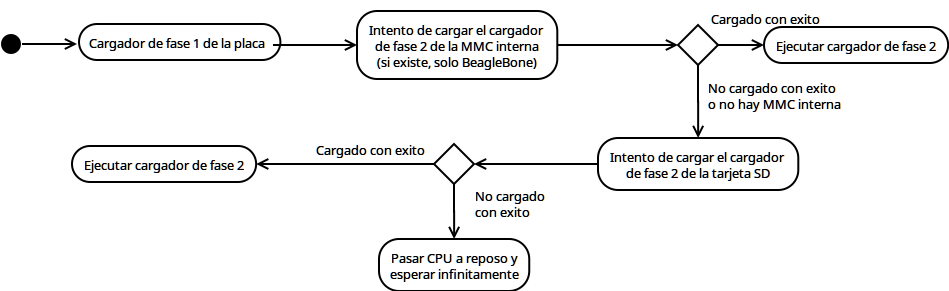
\includegraphics[scale=0.44]{images/stage1_boot_sequence}
	\caption{Secuencia de arranque de primera fase, caso normal}
\end{figure}

\section{El proceso de arranque de Linux}
Una vez ejecutado el Kernel, tras localizar los ficheros cargados en memoria por U-Boot y realizar tareas varias de inicialización, el Kernel descomprime a memoria y monta el initramfs si se ha proporcionado (o en caso contrario, monta el sistema de archivos indicado en la cmdline) y busca el archivo /init en la raíz del sistema de archivos raíz. Una vez encontrado el archivo, lo ejecuta. El archivo puede ser o bien un binario o bien un script cuyo interprete se encuentre en el sistema de archivos.

En caso de que no se encontrara /init, el kernel da un error y pasa la CPU a reposo o se reinicia dependiendo de su configuración. En Linux el proceso inicial (init o PID1) es especial, no puede ser terminado y en caso de que ocurra algún problema que fuerce su terminación o impida su ejecución el sistema operativo se apaga y muestra un error (kernel panic).

Aunque el comportamiento de /init depende de lo que este programado en el, generalmente en este punto se suelen montar los sistemas de archivos que queden por montar y se pide al usuario la clave de cifrado si alguno de los sistemas de archivos esta cifrado. En caso de que se este usando initramfs, se monta el sistema de archivos raíz real y se ejecuta una llamada de sistema llamada ``pivot\_root'', que intercambia el sistema de archivos inicial con el raíz y monta el inicial en una carpeta dentro del nuevo sistema de archivos raíz, que generalmente se suele desmontar inmediatamente liberando la memoria que consumía.

Una vez montado el sistema de archivos raíz real, /init utiliza la llamada de sistema ``execve'' para intercambiarse con el que sera el proceso init desde ese momento, que generalmente se localiza en /sbin/init.

Una vez en ejecución /sbin/init realiza el resto de tareas necesarias para poner el sistema en funcionamiento, principalmente iniciar servicios y consolas (ttys).

En este proyecto, un script de shell cumplirá el rol de /init, y BusyBox cumplirá el rol de /sbin/init.

\section{El proceso de carga de binarios en Linux y libc}
Todo proceso en Linux, excepto el primero (init), comienza cuando otro proceso ya existente utiliza la llamada de sistema ``fork'' para duplicarse.

Una vez duplicado el proceso, uno de los dos sigue ejecutándose (el padre, aquel cuyo identificador de proceso o PID no ha cambiado), mientras que el otro (el hijo) utiliza la llamada de sistema ``execve'' para reemplazarse a si mismo con otro fichero ejecutable.

El Kernel, tras recibir la llamada execve, lee el fichero ejecutable y busca determinados patrones en el inicio del fichero (magic strings) para determinar que de que formato ejecutable se trata. (e.g. si comienza por ``\#!'' seguido por una ruta de un fichero y un salto de linea, es un script.)

Una vez determinado el formato de un fichero, si es un script utiliza la ruta del script como parámetro y ejecuta al interprete, y en caso de ser un binario ejecuta el propio binario.

Si es un binario, generalmente utiliza el formato ELF \cite{elf}, que especifica en la cabecera un programa cargador (ld.so) que carga el binario y todas las librerías enlazadas dinámicamente a este en memoria antes de transferir control al nuevo programa.

Este programa cargador lo proporciona la librería de C que se este utilizando. Debido a que la librería de C cumple esta función, además de ser utilizada por prácticamente todos los programas binarios, es indispensable instalar una librería de C en el sistema operativo para poder utilizarlo.

En este proyecto usaremos EGLibC como librería de C. EGlibC es una divergencia de GLibC (GNU libc) que originalmente se usaba solo para dispositivos embebidos pero posteriormente fue adoptado por varias distribuciones como Debian Linux ya que proporcionaba algunos cambios necesarios.

En la actualidad, las ultimas versiones de GLibC han implementado todos los cambios de EGlibC y EGLibC ya no se mantiene, por lo que se puede decir que ambos se han vuelto a unir como GLibC. Sin embargo para este proyecto utilizaremos versiones algo mas antiguas que tienen mas soporte para este tipo de dispositivos, y por tanto usaremos EGLibC.

\section{El proceso de detección de dispositivos y udev}
El proceso de detección de dispositivos se basa alrededor de un servidor llamado ``udev''. Dicho servidor establece una conexión con el Kernel a través de un socket netlink. Cuando se detecta un cambio en los dispositivos conectados, el Kernel envía por ese socket una cadena de texto llamada ``uevent'' describiendo el cambio en el conjunto de dispositivos.

Udev aplica una serie de reglas configurables por el usuario (en ``/etc/udev/rules.d'') que describen el proceso a aplicar cuando se conecta o desconecta un dispositivo.

Generalmente el proceso consiste en localizar y cargar en el kernel los firmware propietarios que el dispositivo necesite, cargar los módulos que implementen los drivers del dispositivo y crear un nodo de dispositivo en el directorio ``/dev''.

El proceso es configurable y personalizable a través de la carpeta de reglas mencionada anteriormente.

Debido a que necesitamos que la BeagleBoard funcione correctamente si se le conecta por ejemplo un modulo USB WiFi o un teclado inalámbrico, Udev es necesario.

\section{TinyCore}
TinyCore es una distribución de Linux que aspira a mantener un peso mínimo, a ser simple y fácilmente modificable y a no necesitar tener ningún disco conectado para su funcionamiento.

Para cumplir el ultimo requisito, TinyCore opta por no cargar ningún sistema de archivos raíz: cuando se construye TinyCore se crea un initramfs con todos sus componentes, y TinyCore en su /init simplemente configura dicho sistema de archivos inicial para que sea escribible y funciona normalmente desde ahí.

Debido a esto es conveniente minimizar lo máximo posible el peso en disco de TinyCore, ya que el peso de los binarios que normalmente estarían en disco ahora ocupan RAM, que es mucho mas valiosa en un dispositivo como la BeagleBoard.

Anteriormente se ha mencionado a Udev, aunque BusyBox también puede cumplir sus funciones TinyCore esta programado para utilizar Udev, en lugar de reemplazarlo con BusyBox se ha optado por respetar esta decisión para no tener que modificar TinyCore mas de lo necesario.

\section{El interprete de comandos BusyBox}
BusyBox es un interprete de comandos diseñado para dispositivos embebidos. Al contrario que muchos interpretes, que tienen un conjunto reducido de comandos implementados y utilizan binarios externos de otros proyectos para realizar muchas funciones, BusyBox aspira a implementar todo lo posible en un solo binario, optimizando así el uso del espacio en disco.

BusyBox cumple las funciones de ``sh'', de ``util-linux'', de ``init'', y de muchos otros paquetes de software. Como ya se ha mencionado también puede cumplir la función de Udev pero se ha optado a no reemplazar a Udev.

\section{Sistema de gestión de contenedores Docker}
Docker es un sistema de gestión de contenedores que aspira a posibilitar instalar paquetes de software y servidores sin tener que preocuparse de problemas de dependencias, diferencias de distribución de Linux, etc.

Esto se hace empaquetando en las imágenes de los contenedores todas las dependencias y paquetes de la distribución necesarios para el funcionamiento del software. Docker utiliza un modelo de imágenes por capas para minimizar el uso de espacio en disco de contenedores parecidos.

Técnicamente en el contexto de Docker, la tecnología de contenerización se refiere al uso de un sistema de archivos de unión para implementar el modelo de imágenes por capas, el uso de la llamada de sistema ``chroot'' para aislar el sistema de archivos del contenedor de el del anfitrión, el uso de los ``PID namespaces'' para impedir que los contenedores puedan detectar o interferir en los procesos del anfitrión o de los de otros contenedores, el uso de los ``control groups'' para controlar y limitar el uso de recursos de los contenedores y el uso de ``network namespaces'' y ``netfilter'', también llamado ``IPTables'', para virtualizar el subsistema de red del contenedor de el del anfitrión y controlar su acceso al exterior.

La función de Docker es orquestar todas estas tecnologías para que usar un contenedor sea rápido y fácil. Además, Docker proporciona un sistema centralizado en la nube para poder subir y descargar las imágenes que los usuarios vayan creando, así, descargar y ejecutar un software desde la nube generalmente solo necesita un solo comando.

Docker tiene compatibilidad con varios sistemas de archivos de unión, para el proyecto se usara AUFSv3, que es el mas compatible con la versión del Kernel que se usara.

\chapter{Implementación de la solución}
Durante el proyecto se ha desarrollado un script automatizado que genera el sistema operativo desde el código fuente, que es el que se ha usado para generar y probar el proyecto.

Para utilizar dicho script, desde cualquier distribución con Docker instalado, basta ejecutar los siguientes comandos:
\begin{lstlisting}[caption=Uso del build-script]
$ make shell

# En la terminal del contenedor que aparecera:
$ make beaglexm && make

# Si se desea construir una imagen para
# poder flashearla en la BeagleBone:
$ make bbblack && make
\end{lstlisting}
\iffalse $ \fi % Fix syntax highlighting

En este capitulo se describirá el proceso para replicar el proceso que sigue el script y construir manualmente el sistema operativo desde cero.
\section{Entorno de desarrollo}
Para el desarrollo de este proyecto se ha usado Ubuntu Linux versión Trusty (14.04).

Se han instalado los siguientes paquetes:
\begin{lstlisting}[caption=Lista de paquetes]
build-essential bison libncurses5 libncurses5-dev
autoconf gperf flex texinfo wget gawk libtool automake
expat libexpat1-dev bc fakeroot pkg-config dosfstools
git curl ca-certificates xutils-dev
\end{lstlisting}

Adicionalmente se ha cambiado la shell asignada a /bin/sh por bash:
\begin{lstlisting}[caption=Cambio de shell /bin/sh]
# ls -sf /bin/bash /bin/sh
\end{lstlisting}

\section{Compilación del toolchain}
El primer paso para compilar TinyCore a la arquitectura ARM de las placas es compilar un toolchain que emita código
máquina para dicha arquitectura. Se va a utilizar Crosstool-NG para facilitar dicha tarea.
\subsection{Descarga de componentes}
En primer lugar hay que descargar el código fuente de todas las herramientas, que son las siguientes:
\begin{itemize}
	\item GCC: Compilador de C. Se utilizara la versión Linaro 4.8. GCC depende a su vez de las siguientes
	librerías, que también hay que descargar:
	\begin{itemize}
		\item ClooG: Se utilizara la versión 0.18.1.
		\item GMP: Se utilizara la versión 5.1.3.
		\item GNU MPC: Se utilizara la versión 1.0.2.
		\item MPFR: Se utilizara la versión 3.1.2.
		\item ISL: Se utilizara la versión 0.12.2.
	\end{itemize}
	\item GNU Binutils: Herramientas para creación y manipulación de binarios. Utilizadas por GCC y manualmente para
	eliminar símbolos innecesarios de los binarios para reducir su tamaño.
	\item EGLibC: Librería estándar de C, se utilizara la versión 2.13.
\end{itemize}

Una vez descargado todo, la lista de archivos descargados debería coincidir con
la siguiente:

\begin{lstlisting}[language=bash,caption=Lista de tarballs del toolchain]
$ ls -1
binutils-2.22.tar.bz2
cloog-0.18.1.tar.gz
eglibc-2_13.tar.bz2
eglibc-ports-2_13.tar.bz2
gcc-linaro-4.8-2014.01.tar.xz
gmp-5.1.3.tar.xz
isl-0.12.2.tar.bz2
mpc-1.0.2.tar.gz
mpfr-3.1.2.tar.xz
\end{lstlisting}
\iffalse $ \fi % Fix syntax highlighting

\subsection{Descarga del kernel}
Es necesario tener el kernel de Linux descargado para compilar el toolchain ya que se usan algunos
archivos de este. Se utilizara la versión 3.16.5. Una vez descargado hay que descomprimirlo.

\subsection{Descarga y configuración de Crosstool-NG}
Hay que descargar Crosstool-NG de su pagina oficial. Se utilizara la versión
1.20.0. Una vez descargado y descomprimido, hay que ejecutar los siguientes
comandos dentro de su directorio para configurarlo:

\begin{lstlisting}[language=bash,caption=Configuración de Crosstool-NG]
$ cd crosstool_ng_src
$ autoconf
$ ./configure --enable-local
$ make
$ ./ct-ng menuconfig
\end{lstlisting}
\iffalse $ \fi % Fix syntax highlighting

Tras ejecutar el ultimo comando aparece un menú de configuración, visible en la figura 4.1, en este menú
hay que configurar:
\begin{itemize}
	\item La ruta donde están los archivos de las herramientas descargados anteriormente.
	\item El sistema operativo objetivo (Linux), la versión (seleccionar ``custom'' para no descargar dos veces el kernel), y la ruta donde se encuentra el kernel.
	\item La arquitectura objetivo (en este caso es ARM con soporte por hardware para aritmética de punto flotante).
	\item La librería de C a utilizar (eglibc), y su versión. Añadir el parámetro de configuración extra ``--enable-obsolete-rpc''.
	\item El compilador de C/C++ (GCC Linaro) y su versión. Activar también el compilador de C++.
\end{itemize}

\begin{figure}[hb]
	\centering
	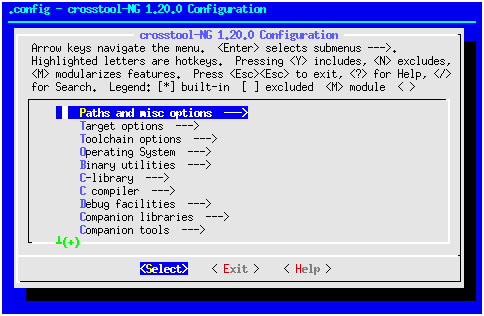
\includegraphics[scale=0.8]{images/ctng_menu}
	\caption{Menú de configuración de Crosstool-NG}
\end{figure}

\subsection{Aplicación de parches}
Un parche o ``patch'' es un archivo que describe la diferencia entre otros dos archivos, generalmente generado con la herramienta ``diff''. Los parches son muy comúnmente usados en entornos de código abierto para enviar a otra persona un cambio del software, o bien se usan varios parches para mantener un conjunto de cambios a través de varias versiones del software que se este modificando (un conjunto de cambios o ``patchset'')

Es necesario aplicar ciertas modificaciones a EGLibC antes de compilarlo para que funcione correctamente en el
dispositivo, de lo contrario algunas aplicaciones darán un error al iniciar. Esto es debido a que, entre otros, hay un error en la versión de EGLibC que estamos usando en ARM por el cual los ejecutables generados apuntan a un ld.so con un nombre distinto al nombre con el que mas adelante se instala en el sistema operativo.

El parche en concreto que resuelve el error mencionado anteriormente ha sido creado por mi. Se ha hallado la localización del código a editar buscando en el código fuente el nombre del cargador que buscaban erróneamente los binarios. Otros parches han sido creados por sus respectivos autores, los cuales generalmente han escrito su nombre en el parche si así lo deseaban, y han sido hallados buscando en internet los errores que iban apareciendo.

Los parches están en el código fuente entregado en la memoria, carpeta ``toolchain/src/ct-ng-patches''. Se aplican enviando a la herramienta patch los contenidos del parche por stdin, i.e. ``cat parche.patch | patch''.

\subsection{Compilación del toolchain}
Una vez preparado todo, ejecutar el siguiente comando para compilar el toolchain. El proceso de compilación tardara
aproximadamente una hora, dependiendo de la potencia de la máquina en la que se haga.
\begin{lstlisting}[language=bash,caption=Compilacion del toolchain]
$ ./ct-ng build
\end{lstlisting}
\iffalse $ \fi % Fix syntax highlighting

\subsection{Configuración del entorno}
Una vez compilado el toolchain, hay que configurar el entorno para usarlo en los pasos posteriores. Para ello hay
que ejecutar los siguientes comandos. Nótese que el entorno solo se configuraría para la ventana de comandos en la que
se ejecute, por lo que habría que realizar los pasos posteriores en dicha ventana o repetir este paso si se usa
otra ventana:
\begin{lstlisting}[language=bash,caption=Configuración del entorno]
$ cd x-tools/arm-unknown-linux-gnueabihf/bin
$ export PATH="$PWD:$PATH"
$ export CROSS_COMPILE="arm-unknown-linux-gnueabihf-"
$ export TARGET="arm-unknown-linux-gnueabihf"
\end{lstlisting}

\section{Compilación del kernel}
\subsection{Modificación del kernel}
Desafortunadamente el kernel de Linux no es totalmente compatible de serie con todos los dispositivos, para que funcione
es necesario parchearlo. Los parches pueden descargarse del repositorio citado en el apartado de referencias \cite{robcnelson}. Tras
copiarlos todos a un directorio junto al del kernel, hay que entrar a la carpeta del kernel y ejecutar los siguientes
comandos:
\begin{lstlisting}[language=bash,caption=Aplicacion de parches del kernel]
$ for p in $PWD/../parches/*.patch; do
    patch -p1 < $p
  done
\end{lstlisting}
\iffalse $ \fi % Fix syntax highlighting

Tambien es necesario instalar AUFSv3 en el kernel. Para ello hay que descargar AUFS \cite{aufs}. AUFS esta compuesto de parches que hay que aplicar (en el directorio raíz, con extensión .patch) y de ficheros que hay que copiar a la fuente del kernel (la carpeta fs y un archivo .h en la carpeta include).

Usar el mismo comando mencionado anteriormente para aplicar los parches.

\subsection{Configuración del kernel}
Una vez parcheado el kernel ya es posible configurarlo. Es conveniente partir de la configuración recomendada en el 
repositorio mencionado anteriormente para acelerar el proceso. Para usar dicha configuración para ello hay que entrar a
la carpeta del kernel y descargar ahí el archivo llamado ``ref\_multi\_v7\_defconfig'', una vez descargado hay que
renombrarlo a ``.config''. Una vez renombrado se puede abrir el menú de configuración con el siguiente comando:

\begin{lstlisting}[language=bash,caption=Configuración del kernel]
$ make ARCH=arm CROSS_COMPILE=$CROSS_COMPILE menuconfig
\end{lstlisting}

Para asegurar el funcionamiento del kernel en el dispositivo hay que activar todas las opciones que controlen la
compilación de cualquiera de los drivers que el dispositivo necesita. Dado que las placas se basan en los SoC OMAP y AM335x una
forma de encontrar todas las opciones relevantes es pulsando el botón ``/'' y escribiendo OMAP y AM335x en el buscador. Otra es prueba y error: con la excepción de la gráfica y lo necesario para el arranque por lo general es posible leer algún mensaje de error describiendo el modulo que falta.

Docker tambien impone una serie de opciones que es necesario activar. Los módulos que exige Docker van cambiando dependiendo de la versión, pero se pueden descubrir pasando cualquier fichero de configuración de kernel a un script llamado checkconfig.sh incluido en el código de Docker, directorio contrib \cite{dockercheckconfig}.

En el código entregado con esta memoria se encuentra una configuración probada en ambos dispositivos.

\begin{figure}[hb]
	\centering
	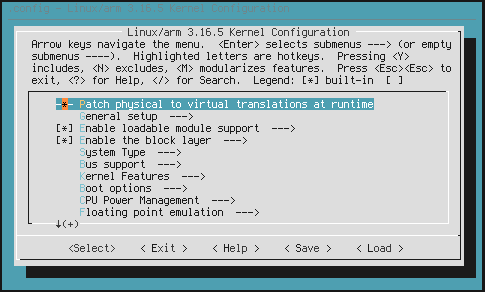
\includegraphics[scale=0.8]{images/kernel_menu}
	\caption{Menú de configuración del kernel}
\end{figure}

\subsection{Compilación del kernel}
Una vez configurado el kernel hay que compilarlo. Debe crearse una carpeta llamada filesystem junto a la del kernel,
esta carpeta sera donde iremos creando el sistema de archivos que usara nuestra versión de TinyCore. Una vez creada
entrar a la carpeta del kernel y compilarlo con el siguiente comando (nótese que el comando se escribe en una sola
linea y se ha dividido en el documento por espacio):

\begin{lstlisting}[language=bash,caption=Compilacion del kernel]
$ make ARCH=arm CROSS_COMPILE=$CROSS_COMPILE
INSTALL_MOD_PATH=$PWD/../filesystem zImage dtbs modules
modules_install
\end{lstlisting}
\iffalse $ \fi % Fix syntax highlighting

\section{Compilación de EGlibC}
Aunque Crosstool-NG ya ha compilado EGlibC para construir el toolchain, hay que compilarlo otra vez para
tener una librería estándar de C en nuestra versión de TinyCore. Para ello descomprimos el tarball que descargamos
anteriormente (``eglibc-2\_13.tar.bz2''). Una vez descomprimido hay que entrar en la carpeta y ejecutar los siguientes
comandos (se presupone que la carpeta filesystem creada anteriormente esta junto a la carpeta de eglibc):

\begin{lstlisting}[language=bash,caption=Compilacion de EGlibC]
$ ./configure --host=arm-unknown-linux-gnueabihf --prefix=/usr
$ make
$ make install_root=$PWD/../filesystem install
\end{lstlisting}

Una vez compilado hay que entrar en la carpeta filesystem y crear un enlace simbólico para que las aplicaciones
puedan encontrar la librería:


\begin{lstlisting}[language=bash,caption=Creacion del enlace simbolico para EGlibC]
$ cd lib
$ ln -s ld-2.13.so ld-linux.so.3
\end{lstlisting}

\section{Compilación de Udev}
Udev es un gestor de dispositivos para Linux, entre sus funciones destacan crear y/o eliminar los nodos de dispositivos en /dev y
cargar firmware propietario del disco (o de la RAM, en el caso de TinyCore, ya que se copia a un tmpfs durante el arranque)
cuando es necesario.
\\\par
Aunque BusyBox puede realizar algunas de las funciones de Udev instalaremos Udev ya que los scripts de TinyCore hacen uso de el,
eliminarlo conllevaría modificar los scripts de TinyCore y ello no entra dentro de los objetivos de este proyecto.
\\\par
Para instalar Udev primero hay que instalar dos dependencias: libusb y usbutils. Empezando por libusb, hay que descargar el código
fuente y descomprimirlo, tras lo cual hay que entrar en la carpeta de libusb y ejecutar los siguientes comandos (se presupone que la carpeta filesystem esta junto a la carpeta de libusb, la primera linea esta dividida por espacio):
\begin{lstlisting}[language=bash,caption=Compilacion de libusb]
$ ./configure --host=arm-unknown-linux-gnueabihf
--prefix=$PWD/../filesystem/usr --disable-udev

$ make
$ make install
\end{lstlisting}

Posteriormente hay que descargar y descomprimir el código de usbutils, tras lo cual hay que entrar en la carpeta de usbutils y
ejecutar los siguientes comandos (la primera linea esta dividida por espacio):

\clearpage

\begin{lstlisting}[language=bash,caption=Compilacion de usbutils]
$ PKG_CONFIG_PATH="$PWD/../filesystem/usr/lib/
pkgconfig:$PWD/../filesystem/usr/share/pkgconfig" ./configure
--host=arm-unknown-linux-gnueabihf
--prefix=$PWD/../filesystem/usr

$ make
$ make install
\end{lstlisting}

Una vez compiladas las dos dependencias, ya se puede compilar udev, para ello, hay que descargar la versión v174 y descomprimirla, tras lo cual hay que entrar en la carpeta y ejecutar los siguientes comandos (la primera linea esta dividida por espacio):

\begin{lstlisting}[language=bash,caption=Compilacion de udev]
$ PKG_CONFIG_PATH="$PWD/../filesystem/usr/lib/
pkgconfig:$PWD/../filesystem/usr/share/pkgconfig" ./configure
--host=arm-unknown-linux-gnueabihf
--prefix=/
--libdir=/lib
--libexecdir=/lib/udev
--includedir=/usr/include
--datarootdir=/usr/share
--with-pci-ids-path=no
--with-systemdsystemunitdir=no
--disable-gudev
--disable-introspection

$ make
$ make DESTDIR="$PWD/../filesystem" install
\end{lstlisting}

\section{Compilación de BusyBox}
Tras descargar y descomprimir el código fuente de BusyBox de su pagina oficial \cite{busybox}, hay que entrar en la carpeta y ejecutar
los siguientes comandos (de nuevo, se presupone que la carpeta filesystem esta junto a la carpeta de BusyBox):

\begin{lstlisting}[language=bash,caption=Compilacion de BusyBox (1)]
$ make ARCH=arm CROSS_COMPILE=$CROSS_COMPILE defconfig
$ make ARCH=arm CROSS_COMPILE=$CROSS_COMPILE
\end{lstlisting}

Posteriormente ejecutar el siguiente comando (el comando esta compuesto de solo una linea pero esta dividido en el documento por espacio)
\begin{lstlisting}[language=bash,caption=Compilacion de BusyBox (2)]
$ make ARCH=arm CROSS_COMPILE=$CROSS_COMPILE
CONFIG_PREFIX=$PWD/../filesystem install
\end{lstlisting}
\iffalse $ \fi % Fix syntax highlighting

\section{Compilación de U-Boot}
\subsection{Modificación de U-Boot}
Al igual que el kernel, es necesario aplicar una serie de parches en U-Boot para su correcto funcionamiento en la BeagleBoard, para ello,
tras descargar y descomprimir el código de U-Boot, hay que descargar los parches \cite{ubootpatchomap} \cite{ubootpatchbone}.

Ya que ha sido necesario modificar algunos de los parches por incompatibilidad, se recomienda usar los aportados
con el código del proyecto, directorio ``u-boot/patch''
\\\par
Una vez descargados, hay que entrar en el directorio de U-Boot y ejecutar los siguientes comandos:
\begin{lstlisting}[language=bash,caption=Aplicacion de parches de U-Boot]
$ for p in $PWD/../parches/*.patch; do
    patch -p1 < $p
  done
\end{lstlisting}
\iffalse $ \fi % Fix syntax highlighting

\subsection{Compilación de U-Boot}
Una vez aplicado el parche, ya es posible compilar U-Boot, para ello hay que entrar en el directorio de U-Boot y ejecutar
los siguientes comandos (las lineas demasiado largas están divididas por espacio):
\begin{lstlisting}[language=bash,caption=Compilacion de U-Boot]
# Para la BeagleBoard-xM (solo uno de los dos)
$ make ARCH=arm CROSS_COMPILE=${CROSS_COMPILE}
omap3_beagle_defconfig

# Para la BeagleBone Black (solo uno de los dos)
$ make ARCH=arm CROSS_COMPILE=${CROSS_COMPILE}
am335x_boneblack_defconfig

$ make ARCH=arm CROSS_COMPILE=${CROSS_COMPILE}
\end{lstlisting}

\section{Compilación de Sudo}
Tras descargar y descomprimir el código fuente de Sudo de su pagina oficial \cite{sudo}, hay que entrar en la carpeta y ejecutar
los siguientes comandos:

\begin{lstlisting}[language=bash,caption=Compilacion de Sudo (1)]
$ autoreconf
$ ./configure --host=$TARGET --prefix=/usr
$ make
\end{lstlisting}

Posteriormente ejecutar el siguiente comando:
\begin{lstlisting}[language=bash,caption=Compilacion de Sudo (2)]
$ make DESTDIR=../filesystem install
\end{lstlisting}
\iffalse $ \fi % Fix syntax highlighting

\section{Compilación de IPTables}
Tras descargar y descomprimir el código fuente de IPTables de su pagina oficial \cite{iptables}, hay que entrar en la carpeta y ejecutar
los siguientes comandos:

\begin{lstlisting}[language=bash,caption=Compilacion de IPTables (1)]
$ ./configure --host=$TARGET --prefix=/usr --disable-nftables
$ make
\end{lstlisting}
\iffalse $ \fi % Fix syntax highlighting

Posteriormente ejecutar los siguientes comandos:
\begin{lstlisting}[language=bash,caption=Compilacion de IPTables (2)]
$ make DESTDIR=../filesystem install

$ ln -sf ../sbin/xtables-multi
../filesystem/usr/bin/iptables-xml
\end{lstlisting}
\iffalse $ \fi % Fix syntax highlighting

\section{Compilación de WPA Supplicant}
WPA Supplicant depende de dos librerías: libnl \cite{libnl} y OpenSSL \cite{openssl}.

Es necesario compilar y instalar estas dos librerias para compilar WPA Supplicant.

Una vez descargadas, ejecutar los siguientes comandos:

\clearpage
\begin{lstlisting}[language=bash,caption=Compilacion de WPA Supplicant]
$ cd openssl
$ ./config --prefix=/usr --openssldir=/etc/ssl --libdir=/lib
shared os/compiler:gcc
$ make depend
$ make
$ make INSTALL_PREFIX=../filesystem install

$ cd ../libnl
$ autoreconf
$ ./configure --host=$TARGET --prefix=/usr
$ make
$ make DESTDIR=../filesystem install

$ cd ../wpa_supplicant/wpa_supplicant
$ cp defconfig .config
$ echo "CONFIG_LIBNL32=y" >> .config
$ echo "CFLAGS += -I$PWD/../../filesystem/usr/include"
>> .config

$ echo "CFLAGS += -I$PWD/../../filesystem/usr/include/libnl3"
>> .config

$ echo "LDFLAGS += -L$PWD/../../filesystem/usr/lib" >> .config

$ LIBDIR=/usr/lib INCDIR=/usr/include BINDIR=/usr/sbin
PKG_CONFIG_PATH="$PWD/../../filesystem/usr/lib/pkgconfig:$PWD/
../../filesystem/usr/share/pkgconfig"
make CC=${CROSS_COMPILE}gcc

$ LIBDIR=/usr/lib INCDIR=/usr/include BINDIR=/usr/sbin
make DESTDIR=$PWD/../../filesystem install
\end{lstlisting}
\iffalse $ \fi % Fix syntax highlighting

\section{Scripts y binarios de TinyCore}
\subsection{Extracción de scripts de TinyCore}
La distribución TinyCore incluye una serie de scripts que controlan el proceso de arranque y el sistema de extensiones
de TinyCore. Dado que su autor construye la distribución manualmente, estos scripts no están en ningún repositorio
fácilmente accesible, sino que hay que extraerlos manualmente de una imagen ya hecha de TinyCore. Para ello hay que
descargar la ISO de Core (la versión mínima de TinyCore), extraer el core.gz, copiarlo a una carpeta temporal y
descomprimirlo usando el siguiente comando:

\begin{lstlisting}[language=bash,caption=Descompresion de core.gz]
$ zcat core.gz | cpio -i -H newc -d
\end{lstlisting}
\iffalse $ \fi % Fix syntax highlighting

Una vez descomprimido hay que eliminar todos los binarios que se encuentren, dejando solo la estructura de directorio, los archivos
de configuración y los scripts. Como norma general todos los scripts y archivos de configuración pueden leerse a simple vista
utilizando cualquier editor de texto, mientras que los binarios no.

Cuando estén todos eliminados debe quedar una lista de archivos similar a la siguiente:

{\footnotesize\begin{lstlisting}[language=bash,caption=Lista de archivos a conservar]
+-- dev
+-- etc
|   +-- fstab
|   +-- group
|   +-- gshadow
|   +-- host.conf
|   +-- hostname
|   +-- hosts
|   +-- init.d
|   |   +-- busybox-aliases
|   |   +-- dhcp.sh
|   |   +-- rcS
|   |   +-- rc.shutdown
|   |   +-- services
|   |   |   +-- crond
|   |   |   +-- dhcp
|   |   |   +-- tftpd
|   |   +-- settime.sh
|   |   +-- tc-config
|   |   +-- tc-functions
|   |   +-- tc_noscan.lst
|   |   +-- tc-restore.sh
|   +-- inittab
|   +-- issue
|   +-- ld.so.conf
|   +-- mke2fs.conf
|   +-- modprobe.conf
|   +-- motd
|   +-- mtab -> /proc/mounts
|   +-- nsswitch.conf
|   +-- passwd
|   +-- pcmcia
|   |   +-- config.opts
|   +-- profile
|   +-- profile.d
|   +-- protocols
|   +-- resolv.conf
|   +-- rpc
|   +-- securetty
|   +-- services
|   +-- shadow
|   +-- shells
|   +-- skel
|   +-- sudoers
|   +-- sysconfig
|   |   +-- backup_device
|   |   +-- ntpserver
|   +-- udev
|       +-- rules.d
|           +-- 42-qemu-usb.rules
|           +-- 50-firmware.rules
|           +-- 50-udev-default.rules
|           +-- 55-tc.rules
|           +-- 56-lsusb.rules
|           +-- 60-cdrom_id.rules
|           +-- 60-pcmcia.rules
|           +-- 60-persistent-alsa.rules
|           +-- 60-persistent-input.rules
|           +-- 60-persistent-serial.rules
|           +-- 60-persistent-storage.rules
|           +-- 75-cd-dvd.rules
|           +-- 80-drivers.rules
|           +-- 95-udev-late.rules
+-- home
+-- init
+-- lib
|   +-- udev
|       +-- firmware.sh
+-- opt
|   +-- bootlocal.sh
|   +-- bootsync.sh
|   +-- shutdown.sh
+-- proc
+-- root
+-- run
+-- sbin
|   +-- autologin
|   +-- ctty-hack
+-- sys
+-- tmp
+-- usr
|   +-- bin
|   |   +-- backup
|   |   +-- bbcheck.sh
|   |   +-- bigHomeFiles.sh
|   |   +-- calc
|   |   +-- chkonboot.sh
|   |   +-- cliorx
|   |   +-- exitcheck.sh
|   |   +-- exittc
|   |   +-- filetool.sh
|   |   +-- fromISOfile
|   |   +-- getdisklabel
|   |   +-- getTime.sh
|   |   +-- history
|   |   +-- ldd
|   |   +-- mountables.sh
|   |   +-- ondemand
|   |   +-- provides.sh
|   |   +-- search.sh
|   |   +-- seekWinPartition
|   |   +-- select
|   |   +-- sethostname
|   |   +-- showbootcodes
|   |   +-- tce
|   |   +-- tce-ab
|   |   +-- tce-audit
|   |   +-- tce-fetch.sh
|   |   +-- tce-load
|   |   +-- tcemirror.sh
|   |   +-- tce-remove
|   |   +-- tce-run
|   |   +-- tce-setdrive
|   |   +-- tce-setup
|   |   +-- tce-size
|   |   +-- tce-status
|   |   +-- tce-update
|   |   +-- tc-terminal-server
|   |   +-- text2lp0
|   |   +-- uuid
|   |   +-- version
|   +-- local
|   +-- sbin
|   |   +-- cache-clear
|   |   +-- cd_dvd_symlinks.sh
|   |   +-- fstype
|   |   +-- rebuildfstab
|   +-- share
|       +-- doc
|       |   +-- tc
|       |       +-- release.txt
|       +-- udhcpc
|           +-- default.script
+-- var
    +-- log
\end{lstlisting}}

Esta estructura de archivos y carpetas debe ser copiada a la carpeta ``filesystem'' mencionada anteriormente.

\subsection{Compilación de binarios de TinyCore}
La gran mayoría de los binarios incluidos en TinyCore provienen de otros proyectos que ya se han compilado,
sin embargo hay dos binarios que son exclusivos a TinyCore: ``rotdash'' y ``autoscan-devices''

Para compilar dichos binarios, descargar los ficheros .c correspondientes \cite{tinycorebinaries} y ejecutar los siguientes comandos:
\begin{lstlisting}[language=bash,caption=Compilacion de binarios de TinyCore]
$ ${CROSS_COMPILE}gcc -o rotdash rotdash.c
$ ${CROSS_COMPILE}gcc -o autoscan-devices autoscan-devices.c
\end{lstlisting}

\section{Docker}
\subsection{Compilación de Docker}
Docker es un solo binario y sus desarrolladores recomiendan compilarlo siempre estáticamente, aunque muchas distribuciones lo compilan dinámicamente.

Para obtener binarios para ARM es necesario compilar Docker en una máquina ARM: Docker es muy complejo y tiene muchas dependencias y el proceso de cross-compilación actualmente no funciona si se activa la función de daemon que necesitamos.

Dado que arreglar el proceso de cross-compilación de Docker ha demostrado ser demasiado costoso en tiempo por complejidad y numero de dependencias se ha optado por compilar Docker en una máquina virtual ARM.

Para ello, en una máquina física o virtual ARM con Docker instalado, clonar el repositorio de Docker \cite{dockerrepo} y ejecutar ``make binary''. Una vez compilados, hay que copiarlos a la carpeta ``filesystem''

En el código fuente del proyecto se encuentran los binarios de Docker ya compilados en la carpeta ``docker''.

Del mismo modo, para crear contenedores, se recomienda utilizar la máquina virtual ARM.

Se dan mas detalles sobre la máquina virtual en el anexo correspondiente.

\section{Creación de la imagen para sdcard (BeagleBoard-xM)}
\subsection{Creación del initramfs}
Para crear el initramfs a partir del directorio filesystem, ejecutar este comando (se divide el comando por espacio):

\begin{lstlisting}[language=bash,caption=Creacion del initramfs]
$ (cd filesystem; find . -print0
| cpio -H newc --null -o
| gzip -9) > initramfs
\end{lstlisting}
\iffalse $ \fi % Fix syntax highlighting

\subsection{Creacion del dispositivo loop}
Hay que crear un dispositivo loop en el que construiremos la imagen. Un dispositivo loop es un dispositivo de bloque virtual que guarda su contenido en un archivo, i.e. es un disco duro virtual.

No es necesario que el dispositivo loop sea del mismo tamaño que la tarjeta, solo que sea igual o mas pequeño que ella y lo suficientemente grande como para que quepa el sistema operativo. Cuanto mas pequeño, menos tardara en copiarse a la tarjeta, así que se creara un dispositivo loop de 150MB.

\begin{lstlisting}[language=bash,caption=Creacion del dispositivo loop]
$ dd of=sdcard.img bs=1 seek=153600000 count=0
\end{lstlisting}
\iffalse $ \fi % Fix syntax highlighting

Una vez creado, hay que montarlo:
\begin{lstlisting}[caption=Montado del dispositivo loop]
# losetup --show -f sdcard.img
\end{lstlisting}

Una vez montado el dispositivo loop, hay que usar gparted o cualquier herramienta de particionado para crear dos particiones, una (la primera) debe ser FAT. El tamaño sera 30MB. La segunda debe ocupar el resto del dispositivo loop, y sera tipo Linux. Posteriormente se formateara como ext2.

Una vez particionado, hay que remontar el dispositivo y escanear sus particiones (reemplazar /dev/loop0 con la salida del comando anterior):

\begin{lstlisting}[caption=Remontado del dispositivo loop]
# losetup -d /dev/loop0
# losetup --show -f sdcard.img
# partx -a /dev/loop0
\end{lstlisting}

Una vez remontado, hay que formatear y montar sus particiones.

\begin{lstlisting}[caption=Formateado y montado del dispositivo loop]
# mkfs.msdos -F 16 -I /dev/loop0p1
# mkfs.ext2 /dev/loop0p2
# mount /dev/loop0p1 /mnt/sdcard-fat
# mount /dev/loop0p2 /mnt/sdcard-ext
\end{lstlisting}

Una vez montadas las particiones, hay que copiar los siguientes archivos:
Copiar los archivos MLO y u-boot.img a la raiz de la FAT. Posteriormente crear un
archivo de configuración de U-Boot llamado uEnv.txt con el siguiente contenido (nótese que solo hay dos lineas, se dividen en varias por espacio):
\begin{lstlisting}[caption=uEnv.txt]
bootargs=console=null consoleblank=0 rootfstype=ext2
root=/dev/ram0 noembed drm.debug=7 debug omapdss.debug=1

uenvcmd=echo bb-tinycore load start;
for i in 1 2 3 4 5 6 7 ; do
setenv mmcpart ${i};
setenv bootpart ${mmcdev}:${mmcpart};
if test -e mmc ${bootpart} /boot/zImage; then
load mmc ${bootpart} ${loadaddr} /boot/zImage;
load mmc ${bootpart} ${rdaddr} /boot/initramfs;
setenv rdsize ${filesize};
load mmc ${bootpart} ${fdtaddr} /boot/dtbs/${fdtfile};
bootz ${loadaddr} ${rdaddr}:${rdsize} ${fdtaddr};
fi;
done
\end{lstlisting}

En la partición ext, hay que crear una carpeta llamada ``boot''. En su interior, hay que copiar el kernel, el initramfs, y hay que crear una carpeta llamada dtbs donde se guardaran los dtbs.

El kernel se puede hallar en la siguiente ruta tras compilarlo: ``kernel/arch/arm/boot/zImage''
Los dtbs se pueden hallar en la siguiente ruta tras compilar el kernel: ``arch/arm/boot/dts/*.dtb''

Una vez copiado todo, hay que desmontar las particiones y el dispositivo loop.
\begin{lstlisting}[caption=Desmontado del loop]
# umount /dev/loop0p1
# umount /dev/loop0p2
# losetup -d /dev/loop0
\end{lstlisting}

Una vez cerrado el dispositivo loop, podemos flashearlo a la tarjeta SD utilizando cat. Suponiendo que la tarjeta SD se encuentre en /dev/sdc:
\begin{lstlisting}[caption=Flasheado de la tarjeta SD]
# cat sdcard.img > /dev/sdc
# sync
# blockdev --flushbufs /dev/sdc
\end{lstlisting}

Una vez flasheado podemos sacar la SD y utilizarla en el dispositivo. Si no se va a utilizar la tarjeta SD para flashear la memoria interna, podemos utilizar gparted para expandir la partición ext2 para que ocupe el resto de la tarjeta para asi tener mas espacio libre.

\section{Flasheo de memoria interna (BeagleBone Black)}
La BeagleBone Black asigna siempre el mismo numero de dispositivo a la memoria interna (1) y a la tarjeta SD (0). Sabiendo esto, una vez arrancado el dispositivo con nuestro sistema operativo, es posible flashear la memoria interna con el siguiente comando (reemplazar 153600000 con el tamaño que se le dio al dispositivo loop durante ``Creacion del dispositivo loop''):
\begin{lstlisting}[caption=Flasheo de la memoria interna]
# head -c 153600000 /dev/mmcblk0 > /dev/mmcblk1
\end{lstlisting}

\chapter{Pruebas}
\section{Prueba de arranque}
Con la SD ya preparada, se introduce la SD en el dispositivo y se arranca, pulsando el botón del cargador de arranque para asegurarme que arranca desde la SD.

Tras unos minutos, el sistema arranca satisfactoriamente, mostrando en pantalla la terminal propia de TinyCore (ver figura 5.1).
\begin{figure}[hb]
	\centering
	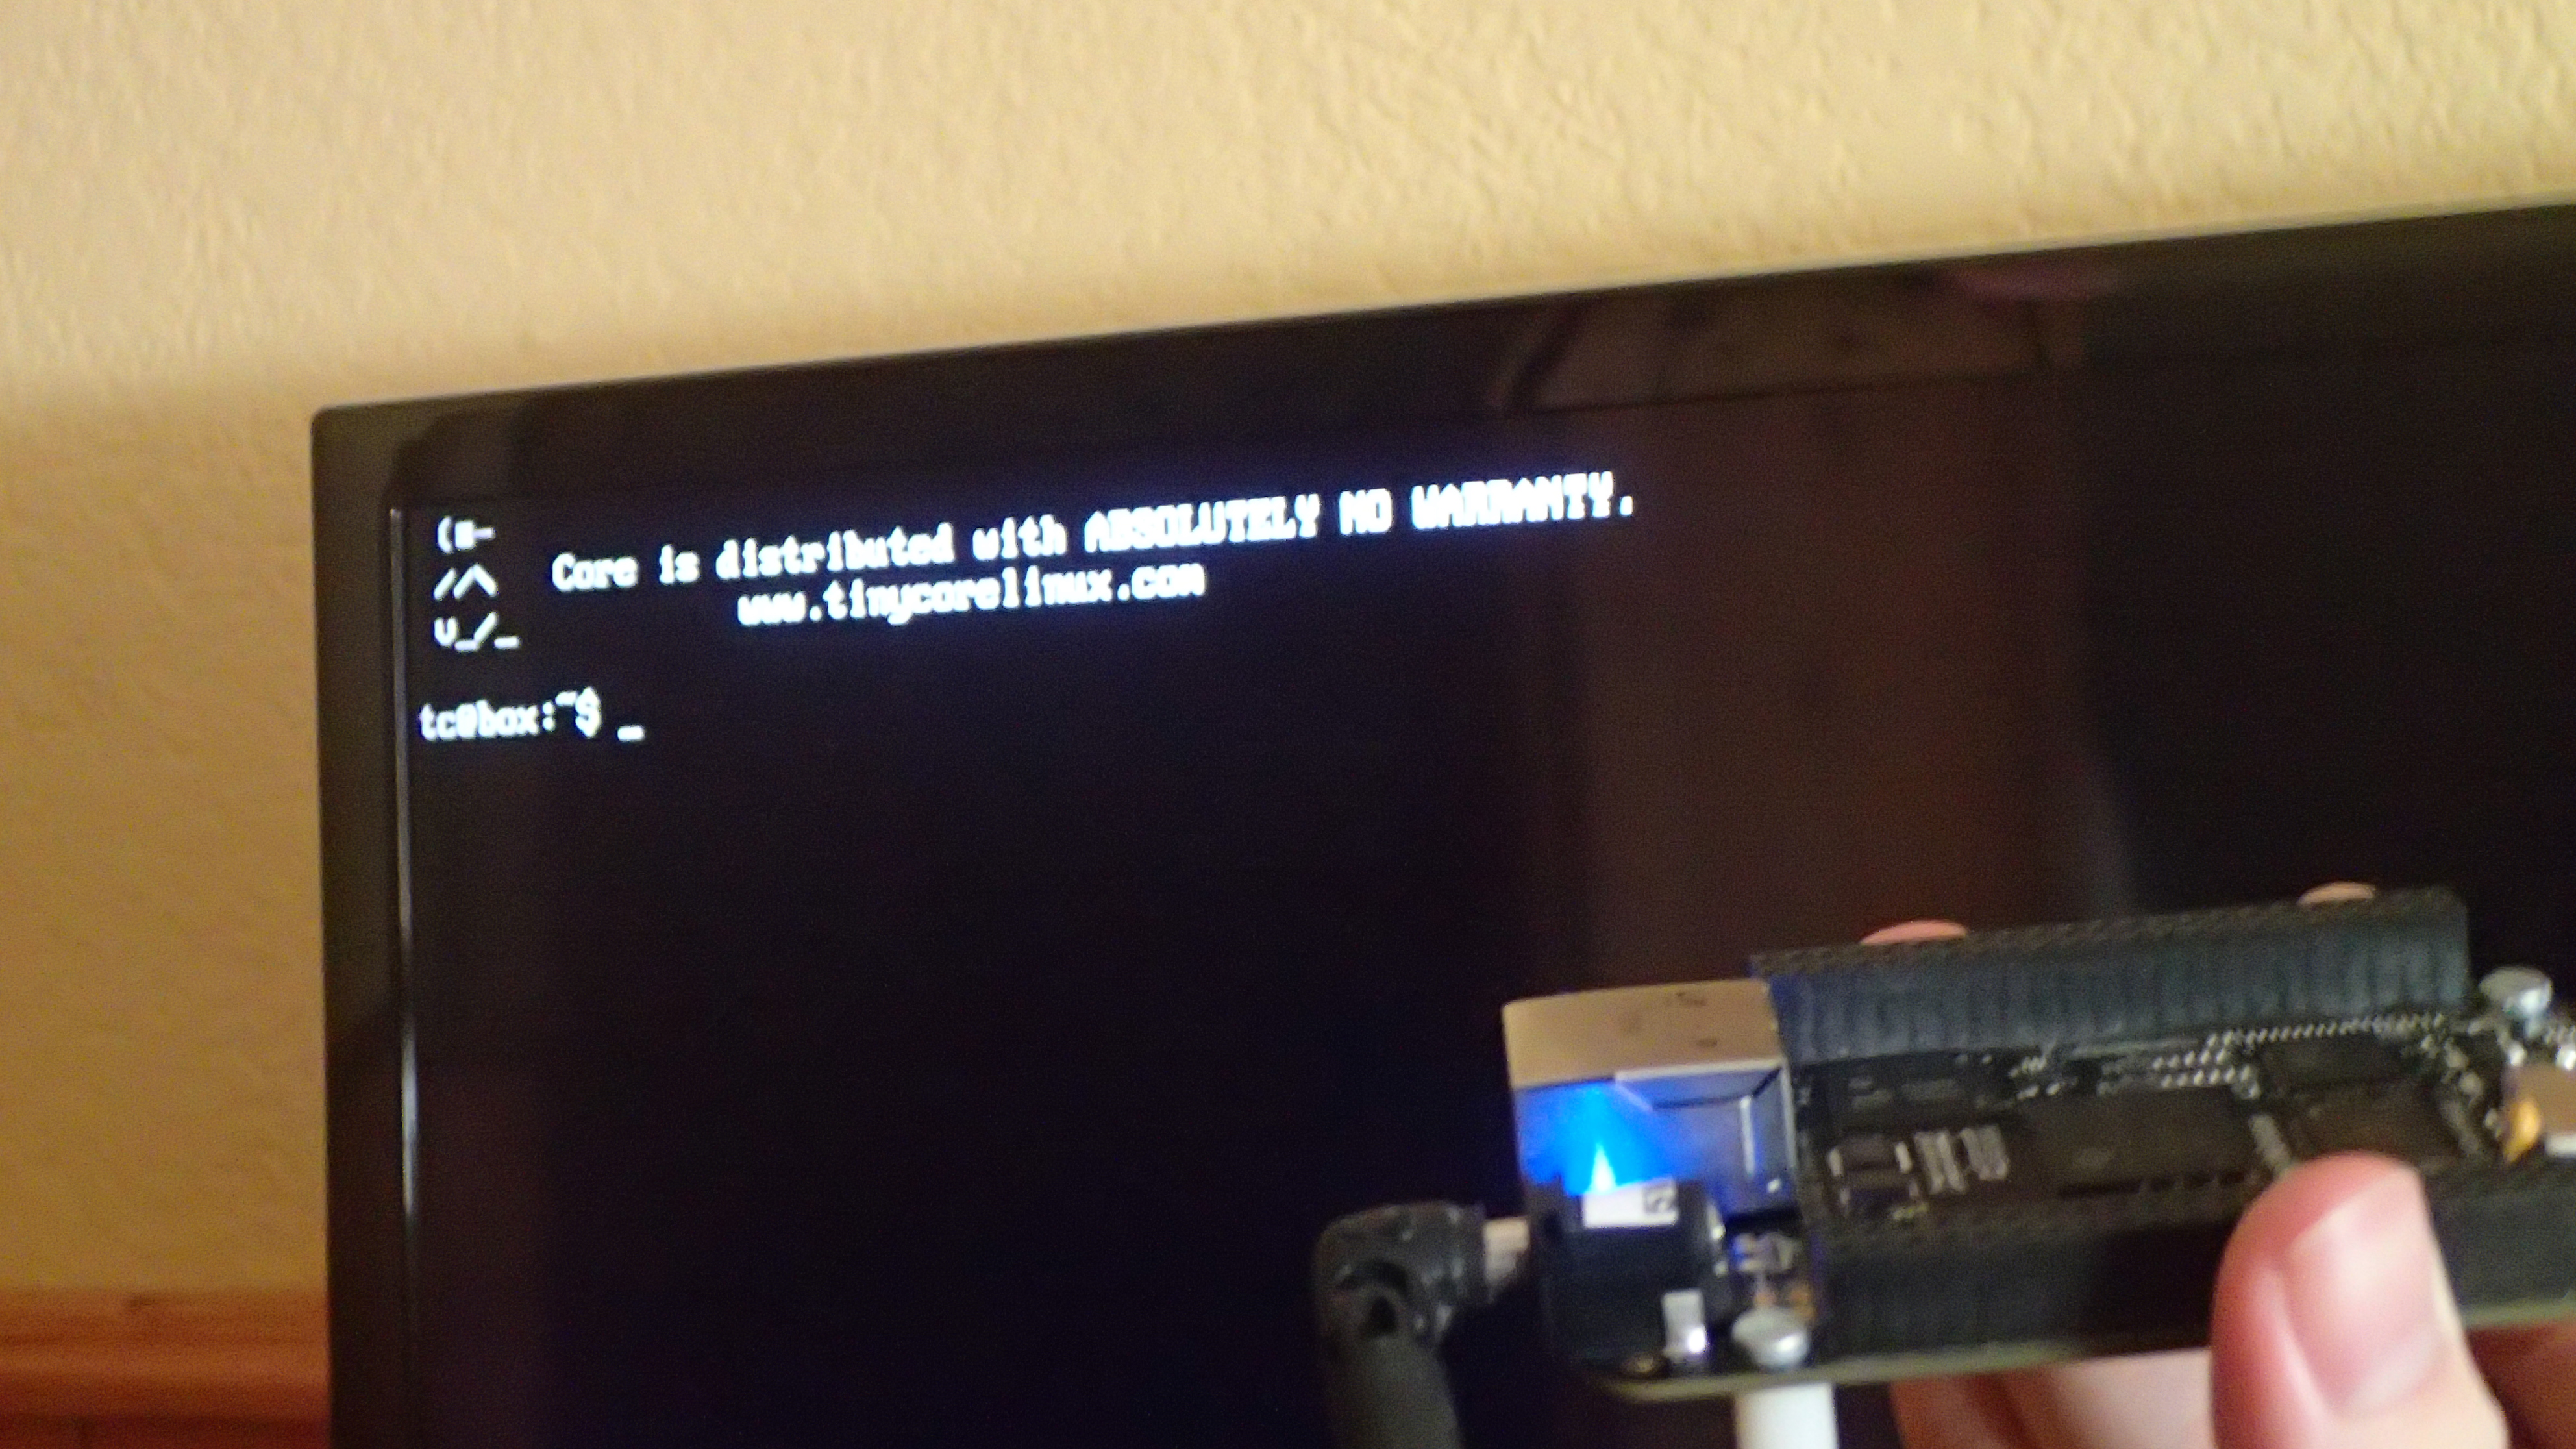
\includegraphics[scale=0.4]{images/boot_test}
	\caption{Prueba de arranque}
\end{figure}

\section{Prueba de conectividad}
Una vez probado el arranque, se prueba la conectividad WiFi. Se ha usado un modulo USB WiFi de la marca BG que utiliza el firmware rt2870.
Para probar la conectividad, se crea un archivo de configuración de WPA Supplicant, y se configura la red con los siguientes comandos:
\begin{lstlisting}[caption=Configuración de red]
# wpa_supplicant -i wlan0 -c wpa.conf &
# udhcpc -i wlan0
\end{lstlisting}

Posteriormente se prueba la conexion a internet descargando una pagina de ejemplo de http://example.org y mostrándola en pantalla (ver figura 5.2):
\begin{lstlisting}[caption=Configuración de red]
$ wget -O - http://example.org | tail -n 10
\end{lstlisting}
\iffalse $ \fi % Fix syntax highlighting

\begin{figure}[hb]
	\centering
	\includegraphics[scale=0.4]{images/wifi_test}
	\caption{Prueba de conectividad}
\end{figure}

\section{Prueba de Docker}
Una vez probada la conectividad, se inicia un contenedor basado en Debian que contiene un servidor gráfico X y un gestor de ventanas ligero llamado Fluxbox. Aparece en pantalla el entorno de escritorio Fluxbox con un fondo de escritorio pre-configurado de Debian. (ver figura 5.3)
\begin{lstlisting}[caption=Inicio del contenedor]
# docker daemon &
# docker run -it --privileged fluxbox startx
\end{lstlisting}

\begin{figure}[hb]
	\centering
	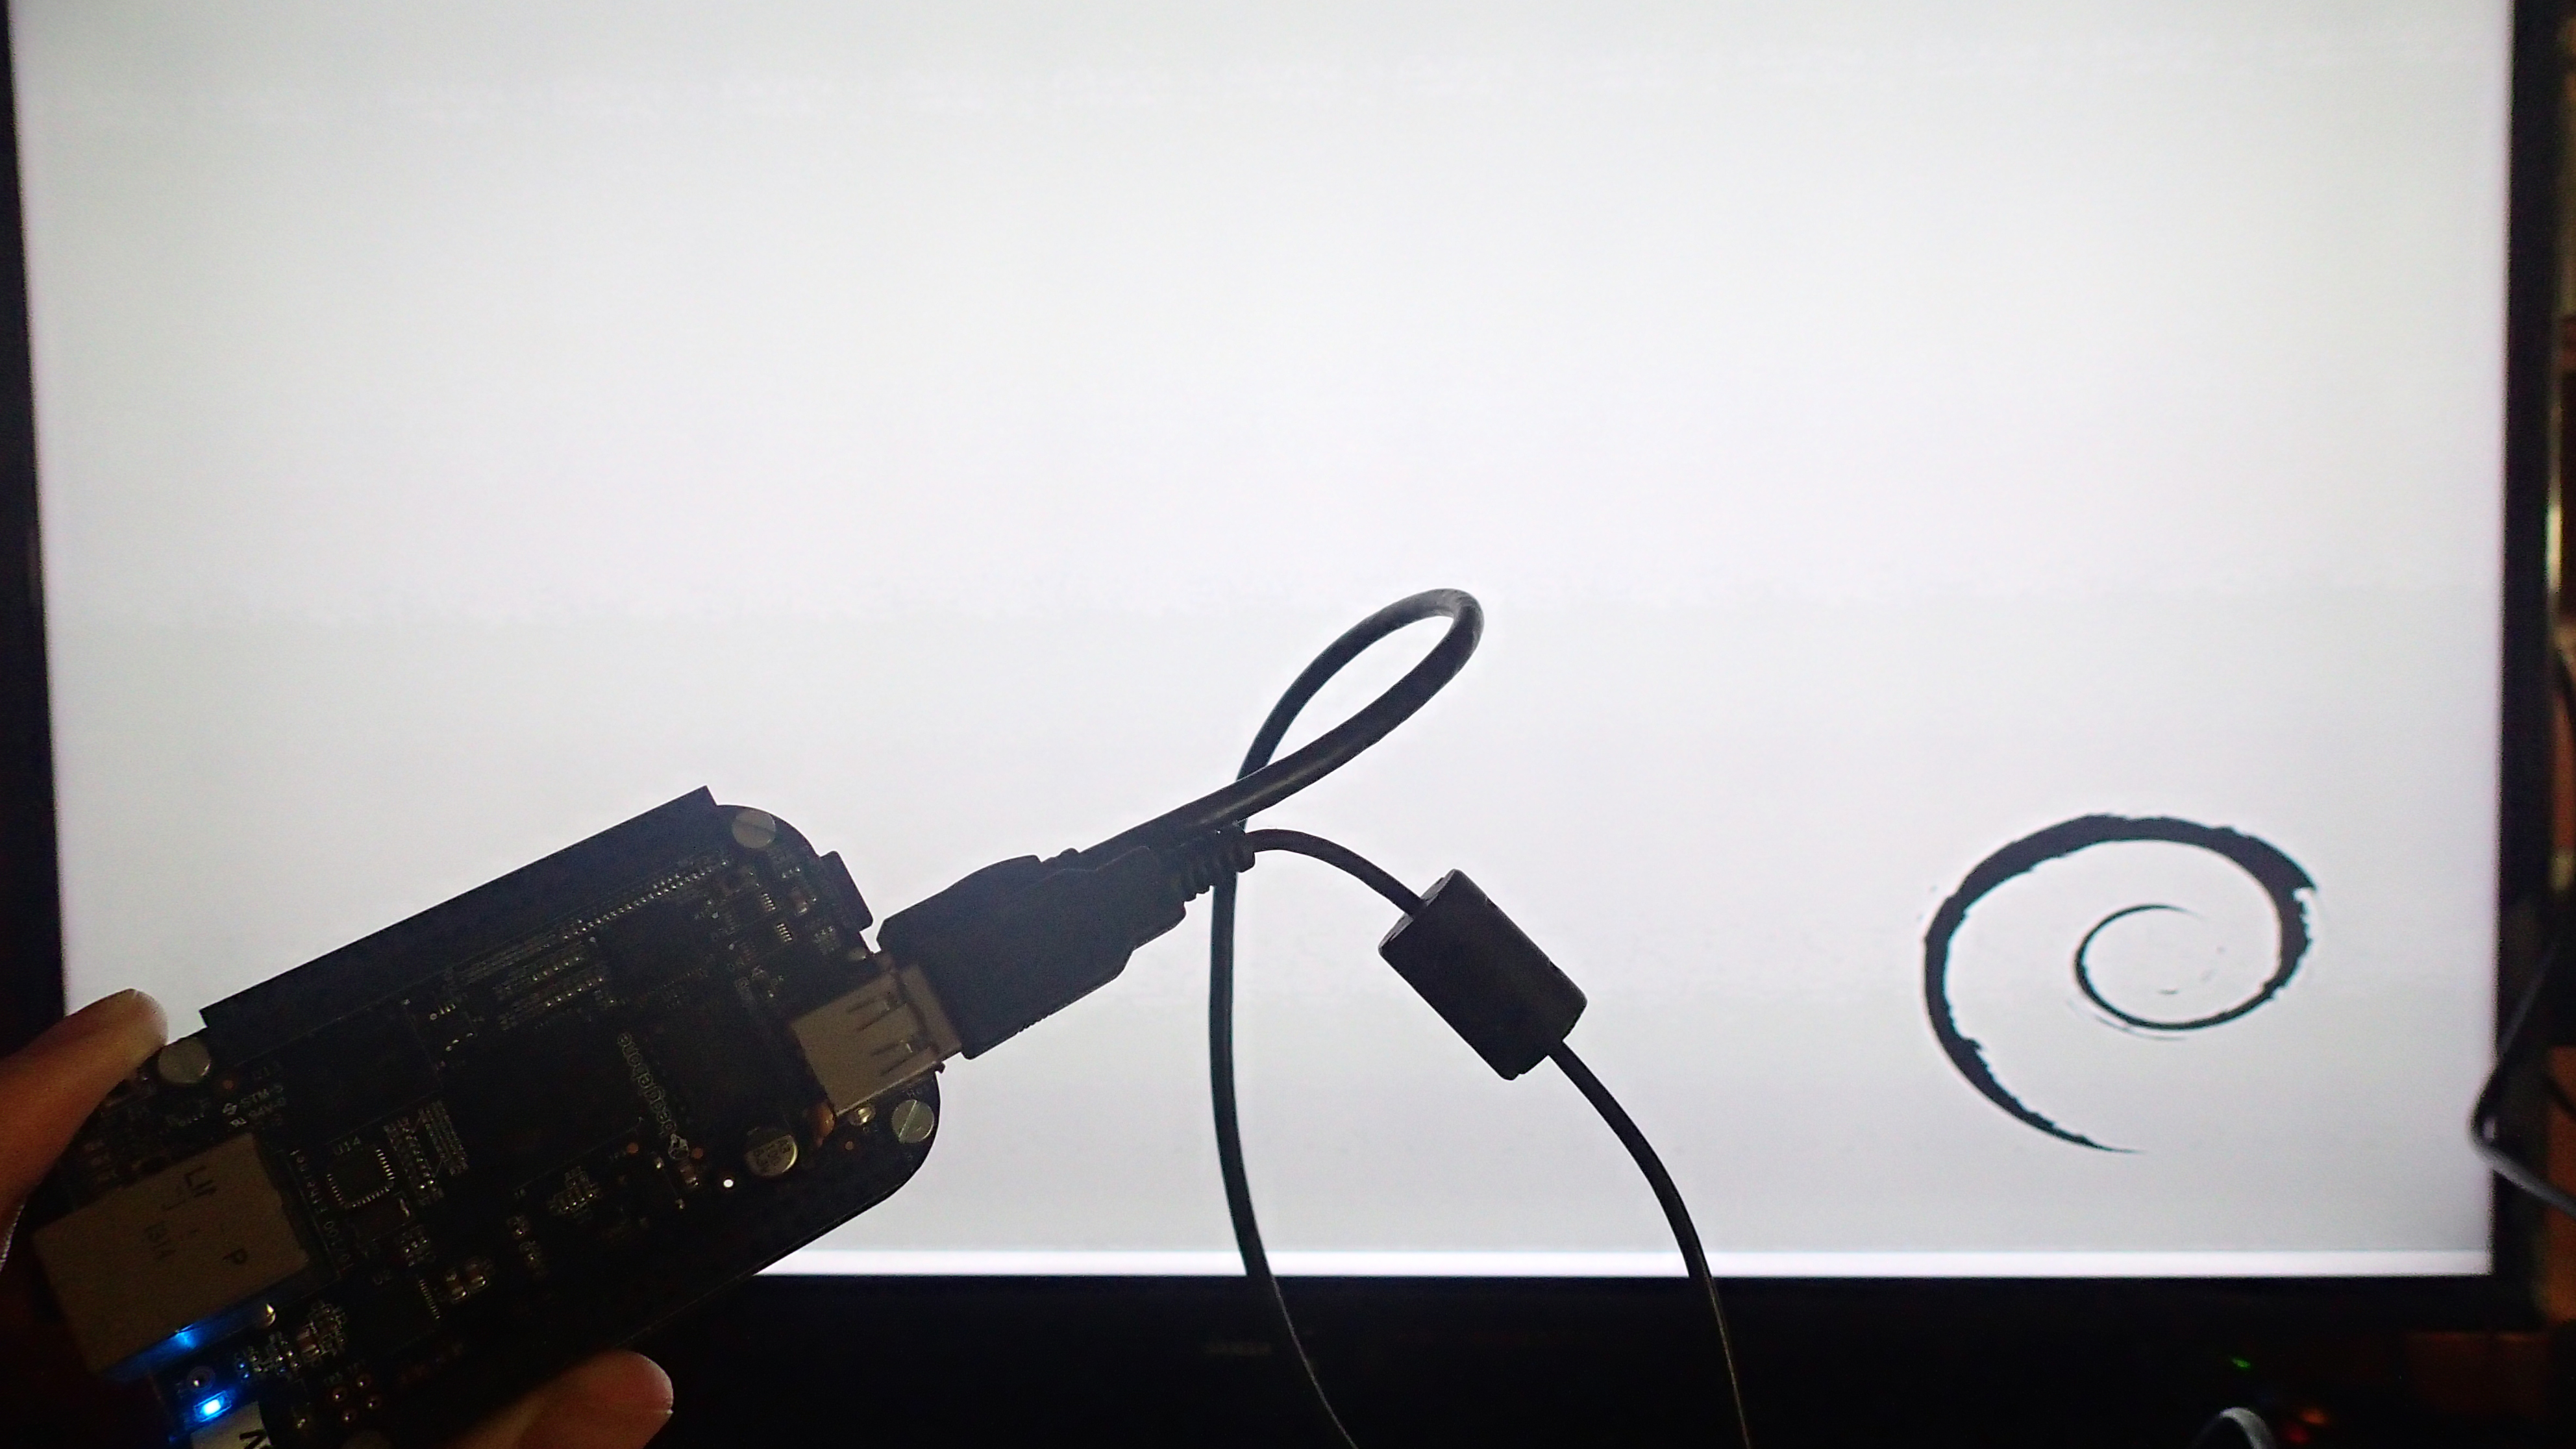
\includegraphics[scale=0.4]{images/docker_test}
	\caption{Prueba de Docker}
\end{figure}


\chapter{Conclusiones}
Tras haber desarrollado el sistema, tenemos una forma de cargar facilmente contenedores con software arbitrario en la BeagleBoard directamente desde la nube o desde una tarjeta SD creada previamente utilizando una máquina virtual.

Como ventajas de este diseño, se puede destacar que ya es innecesario modificar el sistema operativo base de la BeagleBoard pudiendo cargar cualquier software desde un contenedor preparado previamente. Cargar contenedores es muy sencillo y posible de realizar con un solo comando, y construir imágenes de Docker también es muy sencillo. Esto incrementa la accesibilidad de este tipo de plataformas y hace posible desarrollar aplicaciones para estos dispositivos sin necesidad de usar el sistema operativo de fabrica ``Angstrom'' y sin necesidad de hacer un sistema operativo desde cero.

Como inconvenientes de este diseño, hay que destacar los problemas de rendimiento a la hora de crear o instalar imágenes para Docker. Es importante resaltar que el rendimiento es equivalente al nativo una vez el contenedor esta desplegado en el dispositivo.

Sin embargo, dado que instalar imágenes de Docker desde la nube conlleva un paso de descompresión, para imágenes de tamaño considerable como puede ser una distribución estándar de Linux con varios paquetes de software instalados, instalar una imagen desde la nube puede tomar una cantidad considerable de tiempo.

Del mismo modo, la construcción de imágenes de Docker sufre del mismo problema, ya que se deben construir inevitablemente desde un dispositivo o emulador ARM y la descompresión de paquetes software es un paso común dentro de la construcción de dichas imágenes. Se recomienda construir y desplegar las imágenes en un emulador de ARM usando un PC potente para aligerar el proceso, copiando mas tarde la carpeta de datos de Docker a la SD, saltándose así el problema, ya que una vez desplegado el rendimiento es bueno.

Para mi personalmente, además de refrescar mis conocimientos sobre Linux, este proyecto me ha enseñado que el software no se ejecuta en el vacío: por ejemplo, cuando estaba realizando las primeras pruebas, estaba teniendo problemas consiguiendo que el WiFi funcionara de forma estable. Después de intentar todo lo que se me ocurrió: desactivar y reactivar módulos, apagar el DMA de los USBs en la configuración del kernel y recompilar, etc... Me dispuse a desconectar el WiFi USB para probarlo en un ordenador de mesa y me di cuenta de que el WiFi funcionaba mientras tocara con el dedo la parte metálica del conector USB. En el momento que lo soltaba, aunque no hiciera antes ninguna presión, dejaba de funcionar.

La próxima vez que lo probé al día siguiente, no volvió a pasar nada de esto. Especulo que el problema era eléctrico, posiblemente debido a que la fuente de alimentación de la BeagleBoard no tiene toma de tierra.

\chapter{Anexo: Creación de máquina virtual ARM}
Para crear la máquina virtual, en la que instalaremos Debian, en primer lugar necesitamos descargar un kernel, initramfs y dtb para el instalador:
\begin{lstlisting}[caption=Descarga del netinstaller]
# wget http://ftp.debian.org/debian/dists/jessie/
main/installer-armhf/current/images/netboot/initrd.gz

# wget http://ftp.debian.org/debian/dists/jessie/
main/installer-armhf/current/images/netboot/vmlinuz

# wget http://ftp.nl.debian.org/debian/dists/jessie/
main/installer-armhf/current/images/
device-tree/vexpress-v2p-ca15-tc1.dtb
\end{lstlisting}

Posteriormente, debemos instalar el sistema operativo:
\begin{lstlisting}[caption=Instalacion de Debian ARM]
# qemu-system-arm -m 2048M -M vexpress-a15
-dtb vexpress-v2p-ca15-tc1.dtb -cpu cortex-a15
-kernel vmlinuz -initrd initrd.gz
-sd debian-jessie-armhf.img
-append "root=/dev/ram console=ttyAMA0 earlycon"
-no-reboot -nographic
\end{lstlisting}

Una vez arranque la máquina virtual el instalador de Debian es muy sencillo, simplemente pulsar Ok, Siguiente, etc hasta que se instale.

Una vez instalado, hay que sacar el kernel de la máquina virtual para poder pasárselo a QEMU.
\begin{lstlisting}[caption=Extraccion del kernel]
# modprobe nbd max_part=16
# qemu-nbd -c /dev/nbd0 debian-jessie-armhf.img
# mkdir /mnt/nbd0p1
# mount /dev/nbd0p1 /mnt/nbd0p1
# cp /mnt/nbd0p1/initrd.img-3.16.0-4-armmp-lpae .
# cp /mnt/nbd0p2/vmlinuz-3.16.0-4-armmp-lpae .
# umount /mnt/nbd0p1
\end{lstlisting}

Se rearranca la máquina virtual, redirigiendo el puerto local 2222 al puerto de SSH de la máquina virtual:
\begin{lstlisting}[caption=Rearrancado de la máquina virtual]
# qemu-system-arm -m 2048M -M vexpress-a15
-dtb vexpress-v2p-ca15-tc1.dtb -cpu cortex-a15
-kernel vmlinuz-3.16.0-4-armmp-lpae
-initrd initrd.img-3.16.0-4-armmp-lpae
-sd debian-jessie-armhf.img
-append "root=/dev/mmcblk0p2 console=ttyAMA0"
-no-reboot -nographic
-redir tcp:2222::22
\end{lstlisting}

Una vez arrancada, dentro de la máquina virtual hay que instalar SSH y lo necesario para compilar Docker:
\begin{lstlisting}[caption=Instalacion de paquetes]
# apt-get install -y build-essential openssh-server docker.io
\end{lstlisting}

Una vez instalado esto, podemos entrar a la máquina por SSH y copiar archivos de ella:
\begin{lstlisting}[caption=Entrar a la máquina]
# ssh -o port=2222 localhost
\end{lstlisting}
\begin{lstlisting}[caption=Extraer archivos de la máquina]
# scp -r -o port=2222 localhost:/archivo .
\end{lstlisting}

% Esto debe estar al final
\chapter{Referencias}
\renewcommand{\section}[2]{}%
\renewcommand{\chapter}[2]{}%
\begin{thebibliography}{9}
	\bibitem{tinycore} TinyCore: http://distro.ibiblio.org/tinycorelinux/
	\bibitem{docker} Docker: https://www.docker.com/
	\bibitem{crosstoolng} Crosstool-NG: http://crosstool-ng.org/
	\bibitem{beagleboardwiki} BeagleBoard en Wikipedia: https://es.wikipedia.org/wiki/BeagleBoard
	\bibitem{kernelsite} Kernel: http://kernel.org
	\bibitem{udevsrc} Udev: http://ftp.kernel.org/pub/linux/utils/kernel/hotplug/
	\bibitem{busybox} BusyBox: http://busybox.net
	\bibitem{robcnelson} Repositorio de Robert C. Nelson (Parches y configuración del kernel): \\
		https://github.com/RobertCNelson/armv7-multiplatform/tree/v3.16.x/patches
	\bibitem{ubootpatchomap} Parche de U-Boot (BeagleBoard-xM): \\
		https://github.com/RobertCNelson/Bootloader-Builder/blob/master/patches/v2014.10/0001-omap3\_beagle-uEnv.txt-bootz-n-fixes.patch
	\bibitem{ubootpatchbone} Parche de U-Boot (BeagleBone Black): \\
		https://github.com/beagleboard/meta-beagleboard/tree/master/common-bsp/recipes-bsp/u-boot/u-boot-denx
	\bibitem{whatisdocker} What is Docker?: https://opensource.com/resources/what-docker/
	\bibitem{aufs} AUFS: http://aufs.sourceforge.net/
	\bibitem{iptables} IPTables: https://www.netfilter.org/projects/iptables/index.html
	\bibitem{dockercheckconfig} Docker checkconfig.sh: https://github.com/docker/docker/blob/master/contrib/check-config.sh
	\bibitem{dockerrepo} Repositorio Docker: https://github.com/docker/docker
	\bibitem{sudo} Sudo: https://www.sudo.ws
	\bibitem{libnl} libnl: https://github.com/thom311/libnl/releases/download/libnl3\_2\_28/libnl-3.2.28.tar.gz
	\bibitem{openssl} OpenSSL: https://openssl.org/source/openssl-1.0.2h.tar.gz
	\bibitem{tinycorebinaries} Binarios TinyCore: http://distro.ibiblio.org/tinycorelinux/3.x/release/src/
	\bibitem{arm} ARM: http://www.arm.com/products/processors/instruction-set-architectures/index.php
	\bibitem{elf} ELF: https://www.uclibc.org/docs/elf-64-gen.pdf
\end{thebibliography}

\end{document}
